\documentclass[11pt]{article}            % Report class in 11 points
\parindent0pt  \parskip10pt             % make block paragraphs
\usepackage{graphicx}
\usepackage{listings}
\graphicspath{ {images/} }
\usepackage{graphicx} %  graphics header file
\begin{document}
\begin{titlepage}
    \centering
  \vfill
    
\includegraphics[width=8cm]{uni_logo.png} \\ 
	\vskip2cm
    {\bfseries\Large
	Artificial Intelligence \\ (CS13217)\\
	
	\vskip2cm
	Lab Report 
	 
	\vskip2cm
	}    

\begin{center}
\begin{tabular}{ l l  } 

Name: & Anam bibi \\ 
Registration \#: & CSU-S15-118 \\ 
Lab Report \#: & 02 \\ 
 Dated:& 16-03-2018\\ 
Submitted To:& Mr. Usman Ahmed\\ 

 %\hline
\end{tabular}
\end{center}
    \vfill
    The University of Lahore, Islamabad Campus\\
Department of Computer Science \& Information Technology
\end{titlepage}


    
    {\bfseries\Large
\centering
	Experiment \# 1 \\

Implementing Tower of Hanoi Problem\\
	
	}    
 \vskip1cm
 \textbf {Objective}\\  To understand and implement the Tower of Hanoi Problem.
 
 \textbf {Software Tool} \\
1. operating system window 10\\
2. sublime version 3.0\\
3. Python\\

\section{Theory }              
The Tower of Hanoi is a mathematical game or puzzle. It consists of three rods, and a number of disks of different sizes which can slide onto any rod. The puzzle starts with the disks in a neat stack in ascending order of size on one rod, the smallest at the top, thus making a conical shape. \\
The objective of the puzzle is to move the entire stack to another rod, obeying the following simple rules:\\
1.	Only one disk can be moved at a time.\\
2.	Each move consists of taking the upper disk from one of the stacks and placing it on top of another stack i.e. a disk can only be moved if it is the uppermost disk on a stack.\\
3.	No disk may be placed on top of a smaller disk.\\ \\
With three disks, the puzzle can be solved in seven moves. 
The minimum number of moves required to solve a Tower of Hanoi puzzle is 2n - 1, where n is the number of disks.

\section{Task}  
\subsection{Procedure: Task 1 }     

\begin{figure*}
\centering
  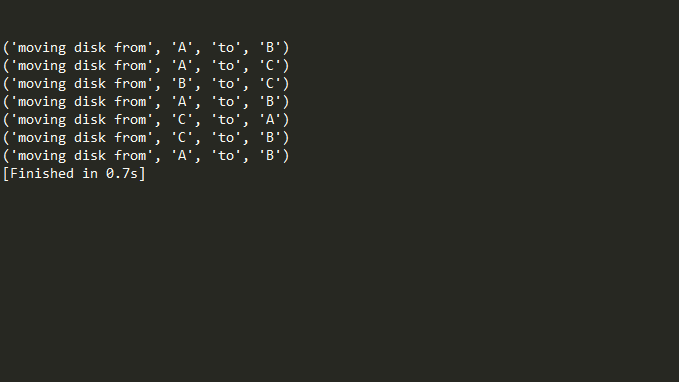
\includegraphics[width=12cm,height=6cm,keepaspectratio]{1.png}
\caption{Time Independent Feature Set}
\label{Figure:3}    
\end{figure*}
The minimum number of moves required to solve a Tower of Hanoi puzzle is 2n - 1, where n is the number of disks.



\begin{lstlisting}[language=Python]

 
def moveTower(height,fromPole, toPole, withPole):
    if height >= 1:
        moveTower(height-1,fromPole,withPole,toPole)
        moveDisk(fromPole,toPole)
        moveTower(height-1,withPole,toPole,fromPole)

def moveDisk(fp,tp):
    print("moving disk from",fp,"to",tp)

moveTower(3,"A","B","C")
\end{lstlisting}

\section{Conclusion}  
The Tower of Hanoi problem can be solved in a variety of ways, with a wide variation in efficiency.According to the legend of the Tower of Hanoi, if one disc was
transferred every second since the beginning of time, it would take about
580 billion years until the puzzle is solved and the world comes to an end.
If this were true, then the world still has many more years to live.
This solution was discovered through the recognition of a recursive
pattern in the puzzle. Through this recursive pattern the function
y=2x-1was created. Using this formula, the number of moves it takes to
solve a 64 disc Tower of Hanoi puzzle was obtained. This function is
useful for obtaining the number of moves for any amount of discs in The
Tower of Hanoi. This is useful when trying to obtain the minimal number
of moves to complete the puzzle as a way to challenge one’s intellectual
strength.


 
\end{document}                          % The required last line
